%-*- coding:utf-8 -*-

\title{ALPS Tutorial \\ 06 -- Application Tutorial (2)}

\begin{document}

\lstset{language={C++},showspaces=false,rulecolor=\color[cmyk]{0, 0.29,0.84,0}}

\begin{frame}
  \titlepage
\end{frame}

\section*{Outline}
\begin{frame}[t,fragile]
   \tableofcontents
\end{frame}

\section{Workflow of ALPS Simulation}
\subsection*{\redm\whiteb\greenb}

\begin{frame}{Workflow of ALPS simulation}
  \begin{center}
    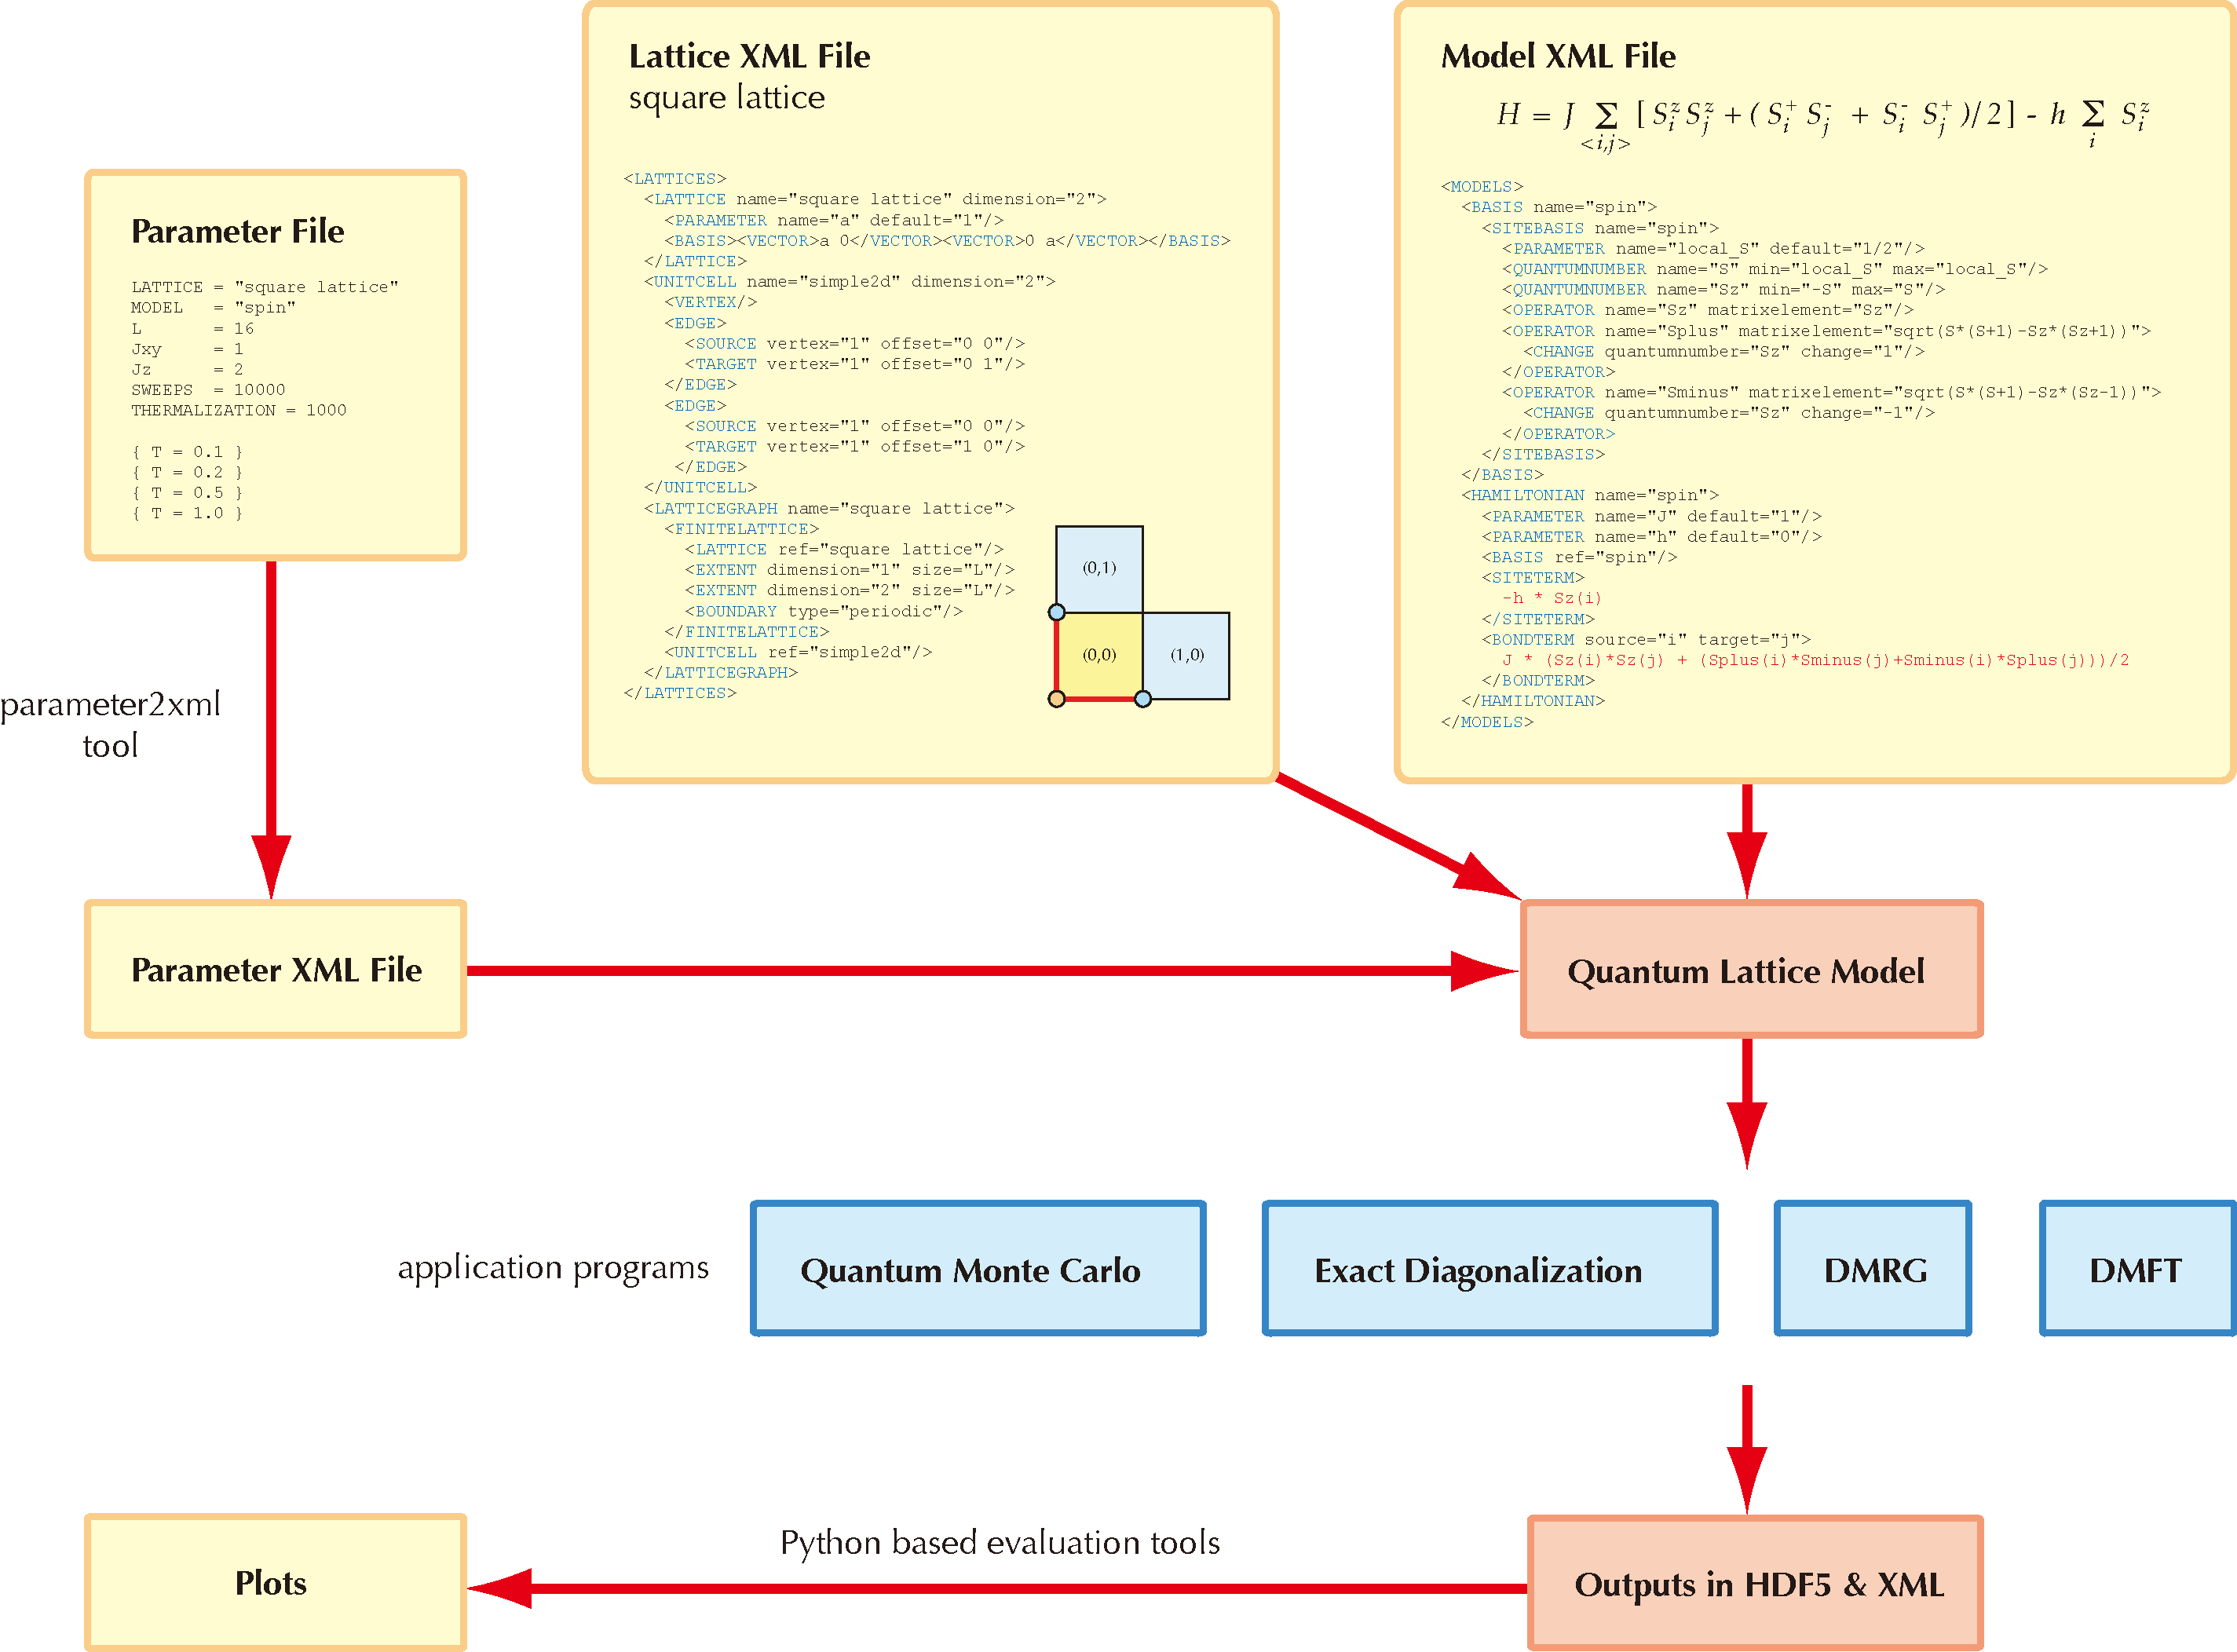
\includegraphics[height=0.8\textheight]{workflow.pdf}
  \end{center}
\end{frame}

\begin{frame}[t,fragile]{ALPS setup script}
  \begin{itemize}
    % \setlength{\itemsep}{1em}
  \item ALPS provides shell script ``{\color {red}alpsvars.sh}'' which initializes environment variables, {\tt ALPS\_HOME}, {\tt PATH}, {\tt LD\_LIBRARY\_PATH}, {\tt PYTHONPATH}, etc
  \item alpsvars.sh can be found in the following places:
    \begin{itemize}
    \item psi.issp.u-tokyo.ac.jp:
      {\footnotesize \tt /opt/MateriApps/alps/alpsvars.sh}
    \item phi.aics.riken.jp:
      {\footnotesize \tt /home/materiapps/alps/alpsvars.sh}
    \item kashiwa.issp.u-tokyo.ac.jp:
      {\footnotesize \tt /home/issp/materiapps/alps/alpsvars.sh}
    \item k.aics.riken.jp:
      {\footnotesize \tt /opt/spire/alps/alpsvars.sh}
    \end{itemize}
  \item For complete list of {\color{red} {\em ALPS-ready} supercomputers} and location of setup script, please refer to \url{https://github.com/wistaria/MateriAppsInstaller}
  \item On \href{http://cmsi.github.io/MateriAppsLive/}{MateriApps LIVE!}, setup script is not needed as environment variables are set by default
  \end{itemize}
\end{frame}

\begin{frame}[t,fragile]
  \frametitle{Preparation for running tutorials}
  \begin{enumerate}
  \item SSH login to workstation
\begin{lstlisting}
$ ssh -YC username@hostname
\end{lstlisting}
  \item Set up environment variables
\begin{lstlisting}
$ source /somewhere/alpsvars.sh
\end{lstlisting}
  \item Confirm that ALPS tools work correctly
\begin{lstlisting}
$ pconfig
\end{lstlisting}
  \item Copy tutorial files
\begin{lstlisting}
$ cp -rp $ALPS_HOME/tutorials $HOME
\end{lstlisting}
  \end{enumerate}
\end{frame}

\begin{frame}[t,fragile]
  \frametitle{Preparation for running tutorials}
  In the case of using ALPS installed in \verb+$HOME+ by yourself
  \begin{enumerate}
  \item Set up environment variables
\begin{lstlisting}
$ source $HOME/alps/bin/alpsvars.sh
\end{lstlisting}
  \item Confirm that ALPS tools work correctly
\begin{lstlisting}
$ pconfig
\end{lstlisting}
  \item Copy tutorial files
\begin{lstlisting}
$ cp -rp $ALPS_HOME/tutorials $HOME
\end{lstlisting}
  \end{enumerate}
\end{frame}

\begin{frame}[t,fragile]
  \frametitle{Preparation for running tutorials}
  In the case of using MateriApps LIVE!
  \begin{enumerate}
  \item Confirm that ALPS tools work correctly
\begin{lstlisting}
$ pconfig
\end{lstlisting}
  \item Copy tutorial files
\begin{lstlisting}
$ cp -rp /usr/share/alps/tutorials $HOME
\end{lstlisting}
  \end{enumerate}
\end{frame}

\begin{frame}[t,fragile]
  \frametitle{Miki's first ALPS simulation}
  \begin{itemize}
    \item Run simulations from Python (\href{http://alps.comp-phys.org/mediawiki/index.php/ALPS_2_Tutorials:MC-02_Susceptibilities}{mc-02-susceptibilities})
\begin{lstlisting}
$ cd $HOME/tutorials/mc-02-susceptibilities
$ python tutorial2a.py
$ python tutorial2b.py
$ python tutorial2c.py
$ python tutorial2d.py
$ python tutorial2full.py
\end{lstlisting}
    \item Everytime you run Python script, plot window will be opened
    \item Python script will finish by closing plot window
    \item The last script will plot all the results in one panel
  \end{itemize}
\end{frame}

\begin{frame}[t,fragile]
  \frametitle{What did I calculate, acutually?}
  \begin{itemize}
  \item Magnetic susceptibility of various antiferromagnetic Heisenberg models as a function of temperature
    \begin{itemize}
    \item tutorial2a.py: classical Heisenberg model on linear chain
    \item tutorial2b.py: classical Heisenberg model on two-leg ladder
    \item tutorial2c.py: quantum ($S=1/2$) Heisenberg model on linear chain
    \item tutorial2d.py: quantum ($S=1/2$) Heisenberg model on two-leg ladder
    \end{itemize}
  \item Questions
    \begin{itemize}
      \item Is there a difference between the classical and quantum calculation?
      \item How does the susceptibility depend on the lattice?
      \item Why does the susceptibility change?
    \end{itemize}
  \end{itemize}
\end{frame}

\section{Preparation of Input Files}
\subsection*{\redm\whiteb\greenb}

\begin{frame}[t,fragile]{Inputs/Outputs of ALPS simulation}
  \begin{itemize}
  \item Typically one ``simulation'' consists of several parameter sets, e.g. different temperatures
    \begin{itemize}
    \item ``Job'': whole simulation.  Set of ``tasks''
    \item ``Task'': calculation for a particular set of parameters.  Set of ``runs''
    \item ``Run'' (or ``clone''): independent calulations on the same parameter set but with different random seeds
    \end{itemize}
  \item XML input/output files (share the same basename)
  \begin{center}
    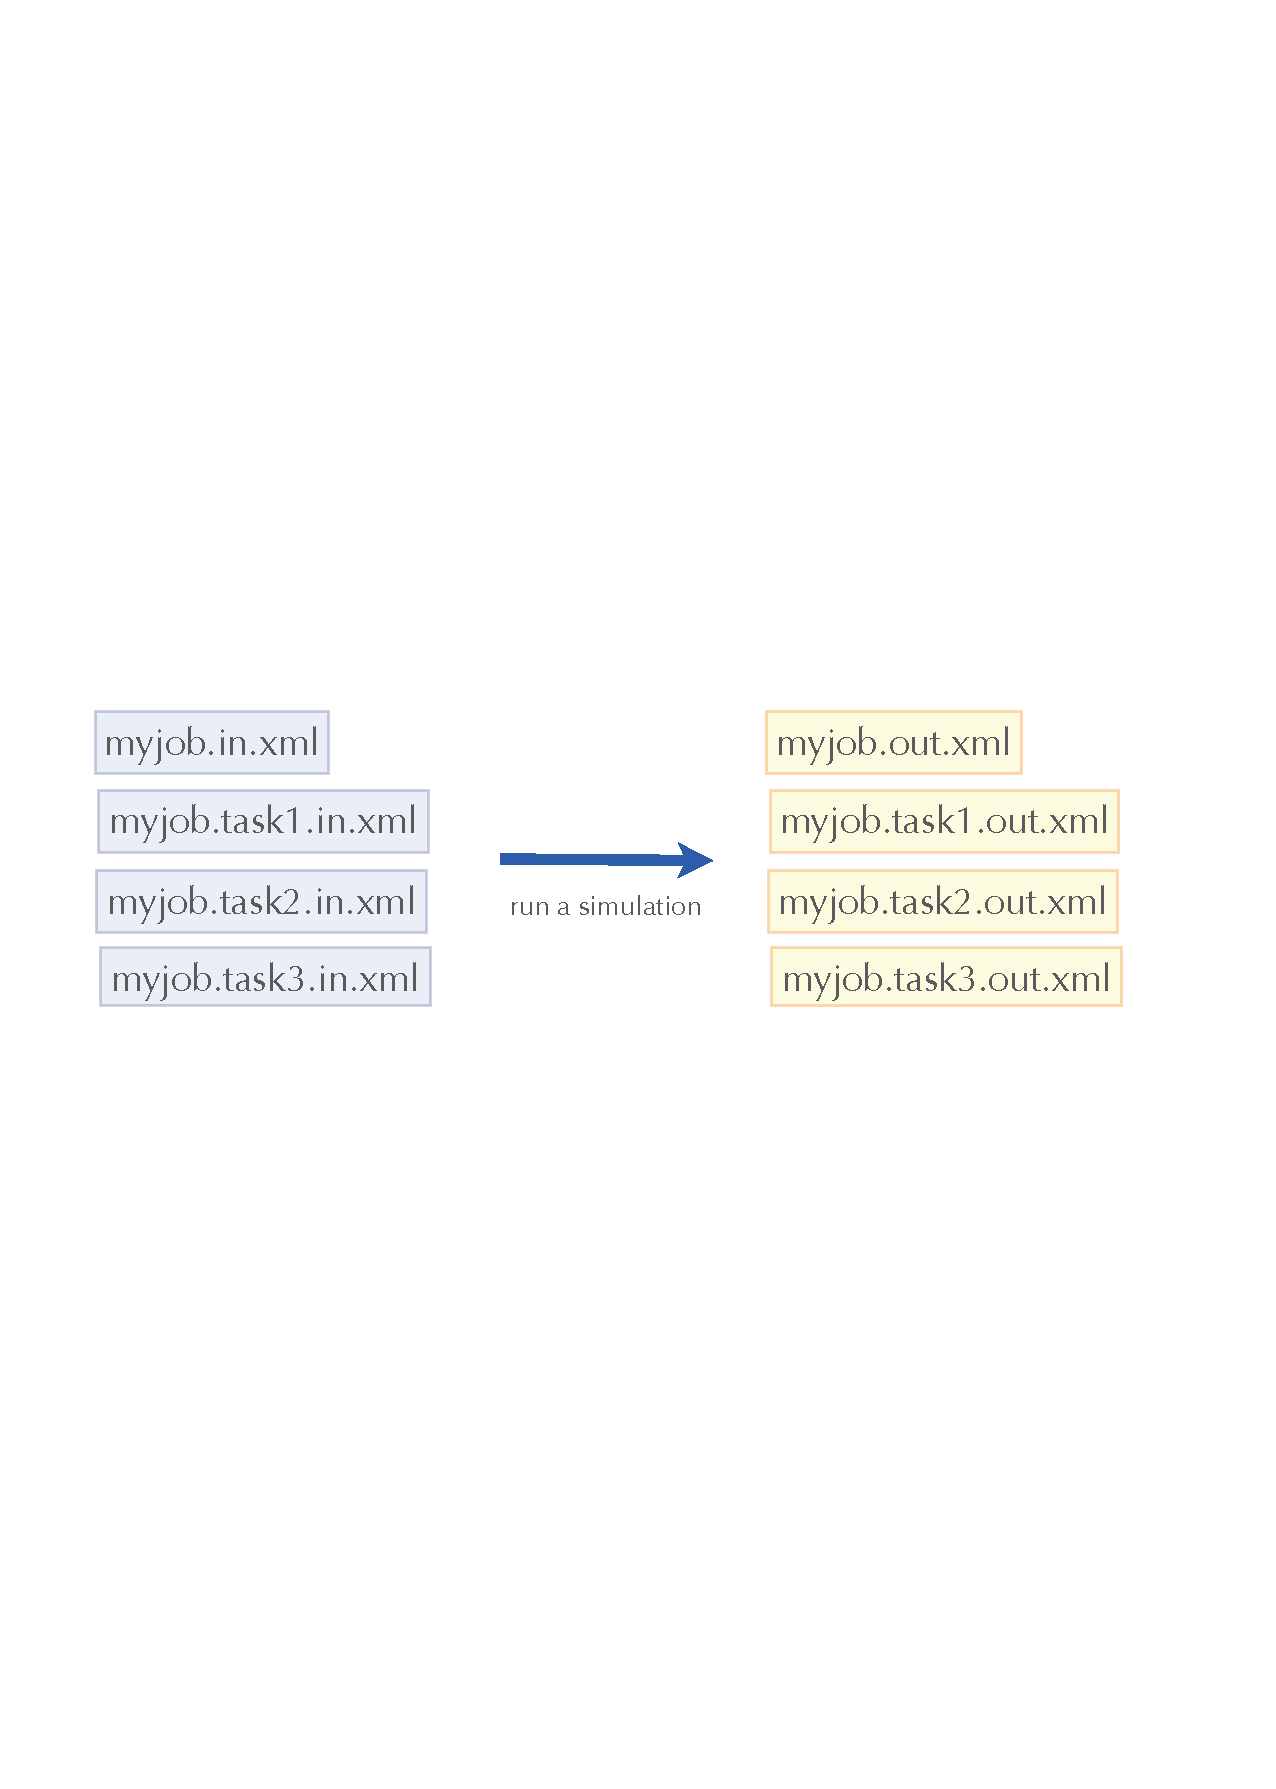
\includegraphics[width=.55\textwidth]{simulation1.pdf}
  \end{center}
  \end{itemize}
\end{frame}

\begin{frame}[t,fragile]{Job XML file (master file)}
  \begin{center}
    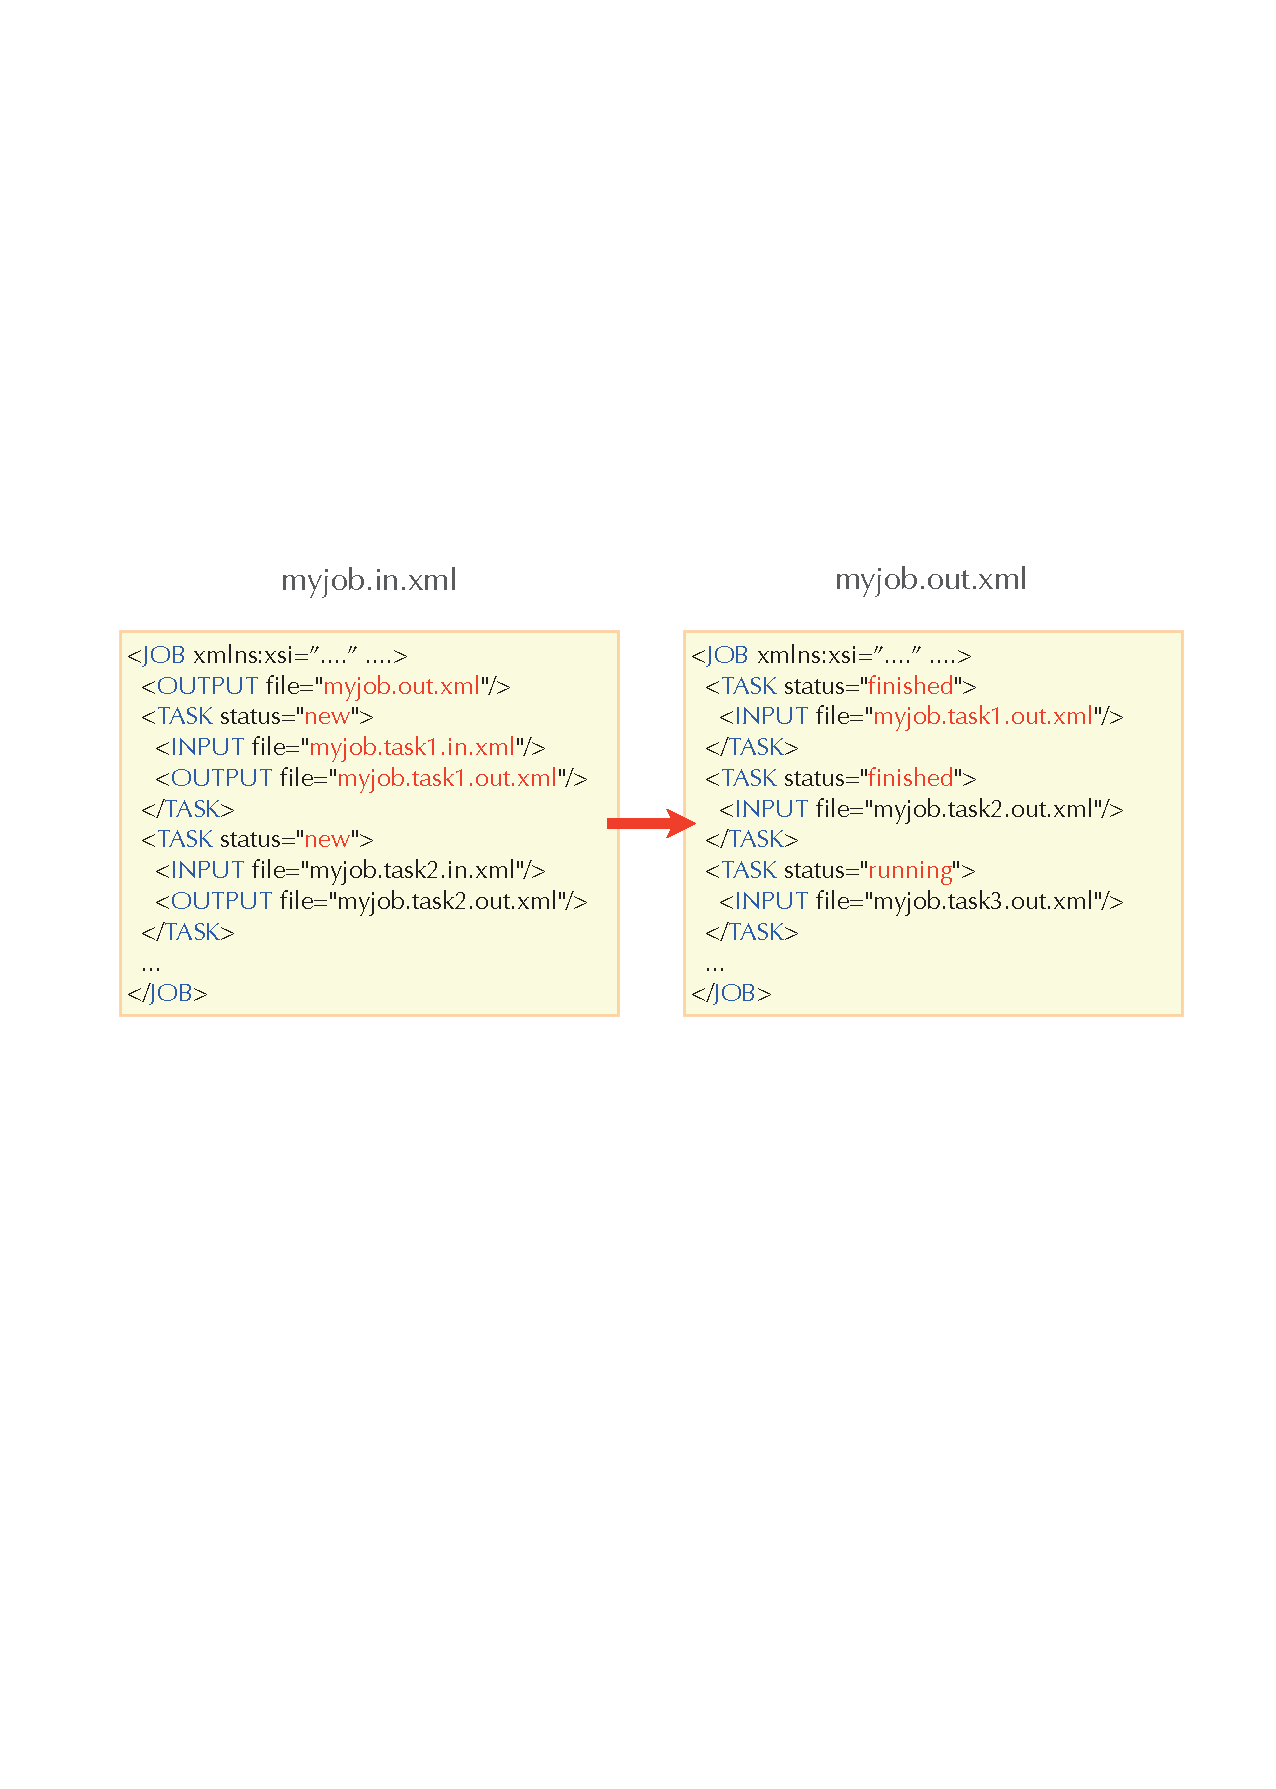
\includegraphics[height=.6\textheight]{simulation2.pdf}
  \end{center}
\end{frame}

\begin{frame}[t,fragile]{Task XML files}
  \begin{center}
    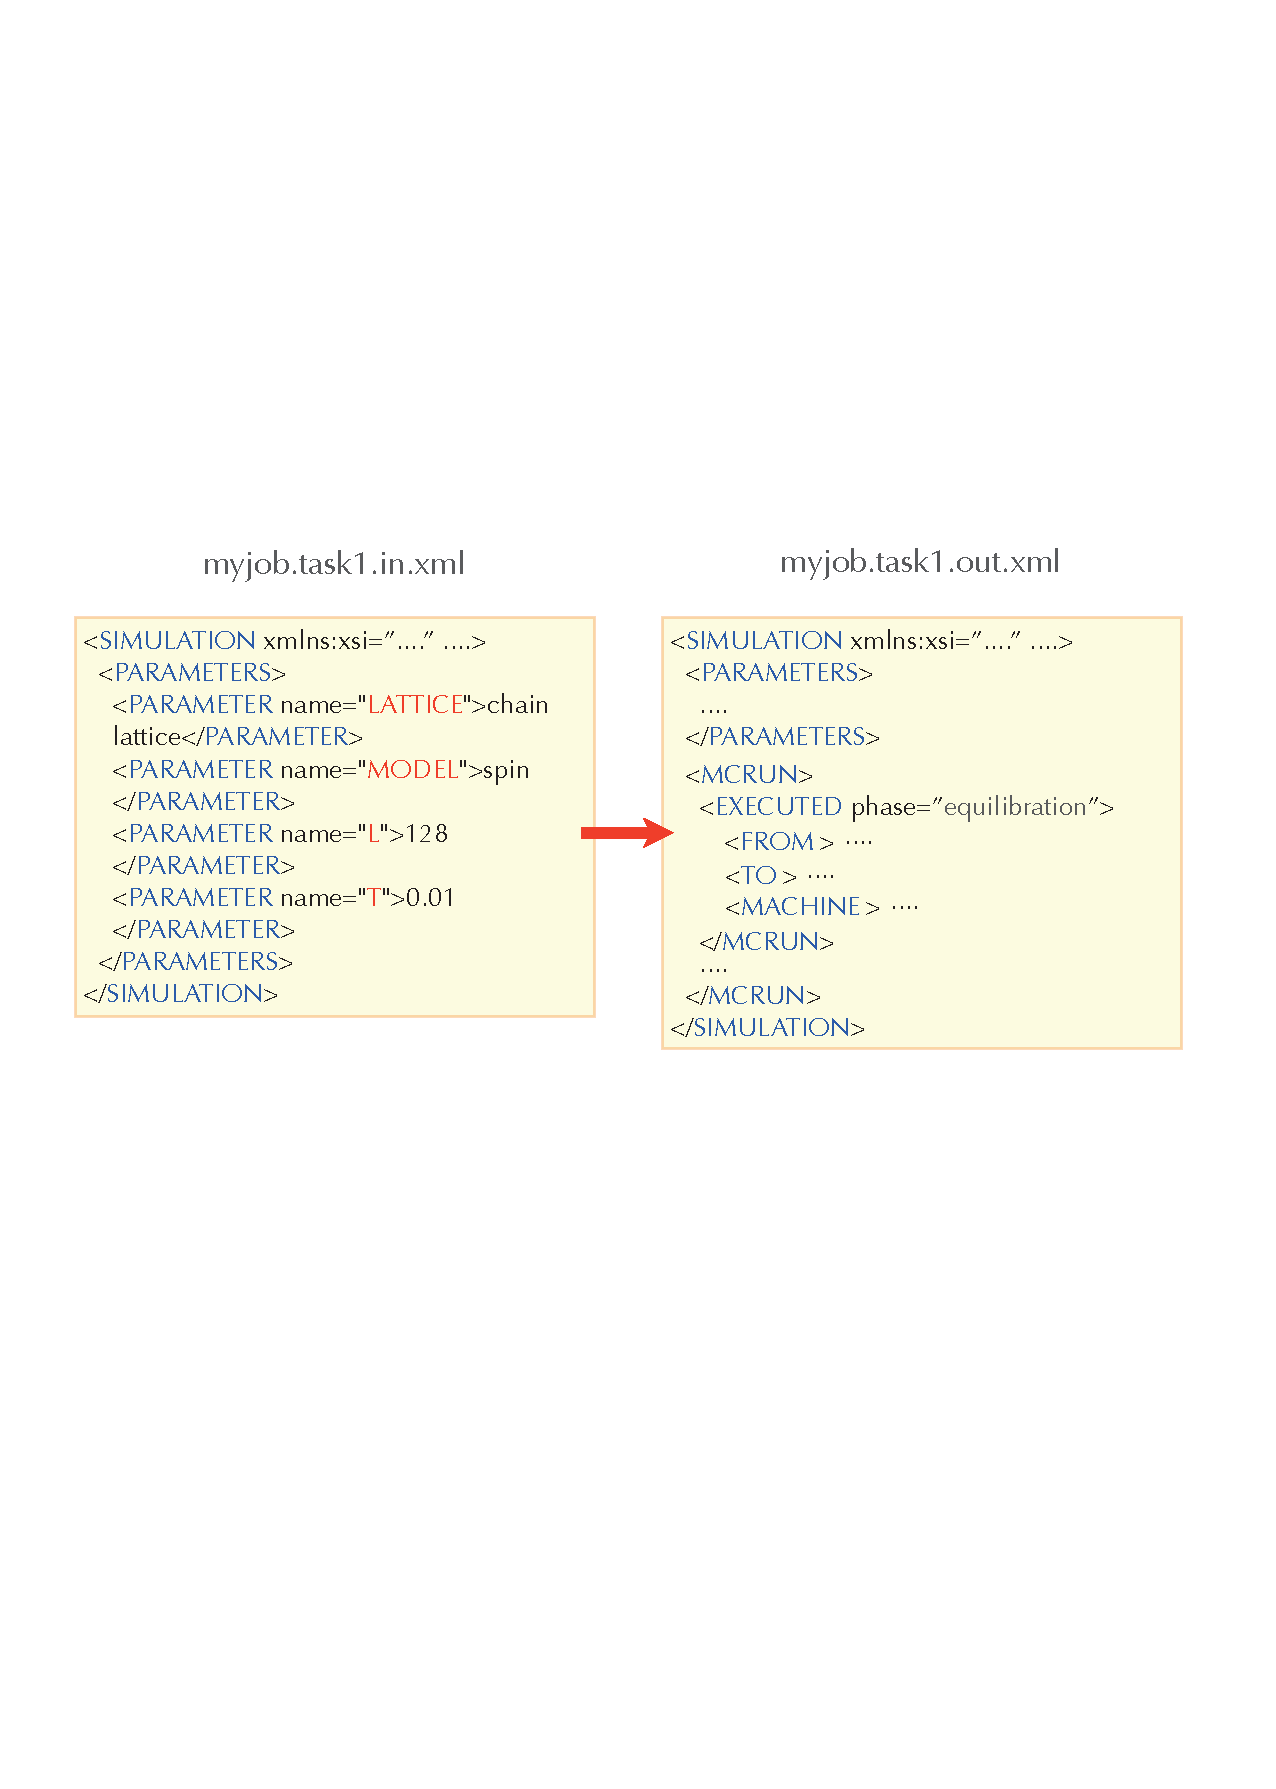
\includegraphics[height=.6\textheight]{simulation3.pdf}
  \end{center}
\end{frame}

\begin{frame}[t,fragile]{Binary files generated by ALPS applications}
  \begin{itemize}
    \setlength{\itemsep}{1em}
  \item HDF5 (extension: {.h5})
    \begin{itemize}
    \item Simulation results and information about excecution (execution time, hostname, etc) will be written HDF5 files for each task
    \item Python evaluation tool reads simulation results from HDF5 files
    \end{itemize}
  \item XDR (extension: {.xdr})
    \begin{itemize}
    \item Checkpoint data (spin configuration, etc) will be saved at a fixed interval (default: 1 hour)
    \item Suspended simulations can be resumed from checkpoints
    \end{itemize}
  \end{itemize}
\end{frame}

\begin{frame}[t,fragile]{Two ways to prepare input files}
  \begin{enumerate}
    \setlength{\itemsep}{1em}
  \item create within Python script: ex) \href{https://github.com/cmsi/alps-tutorial/blob/tutorials/tutorials/mc-02-susceptibilities/tutorial2a.py}{tutorial2a.py}
    %\begin{center}
      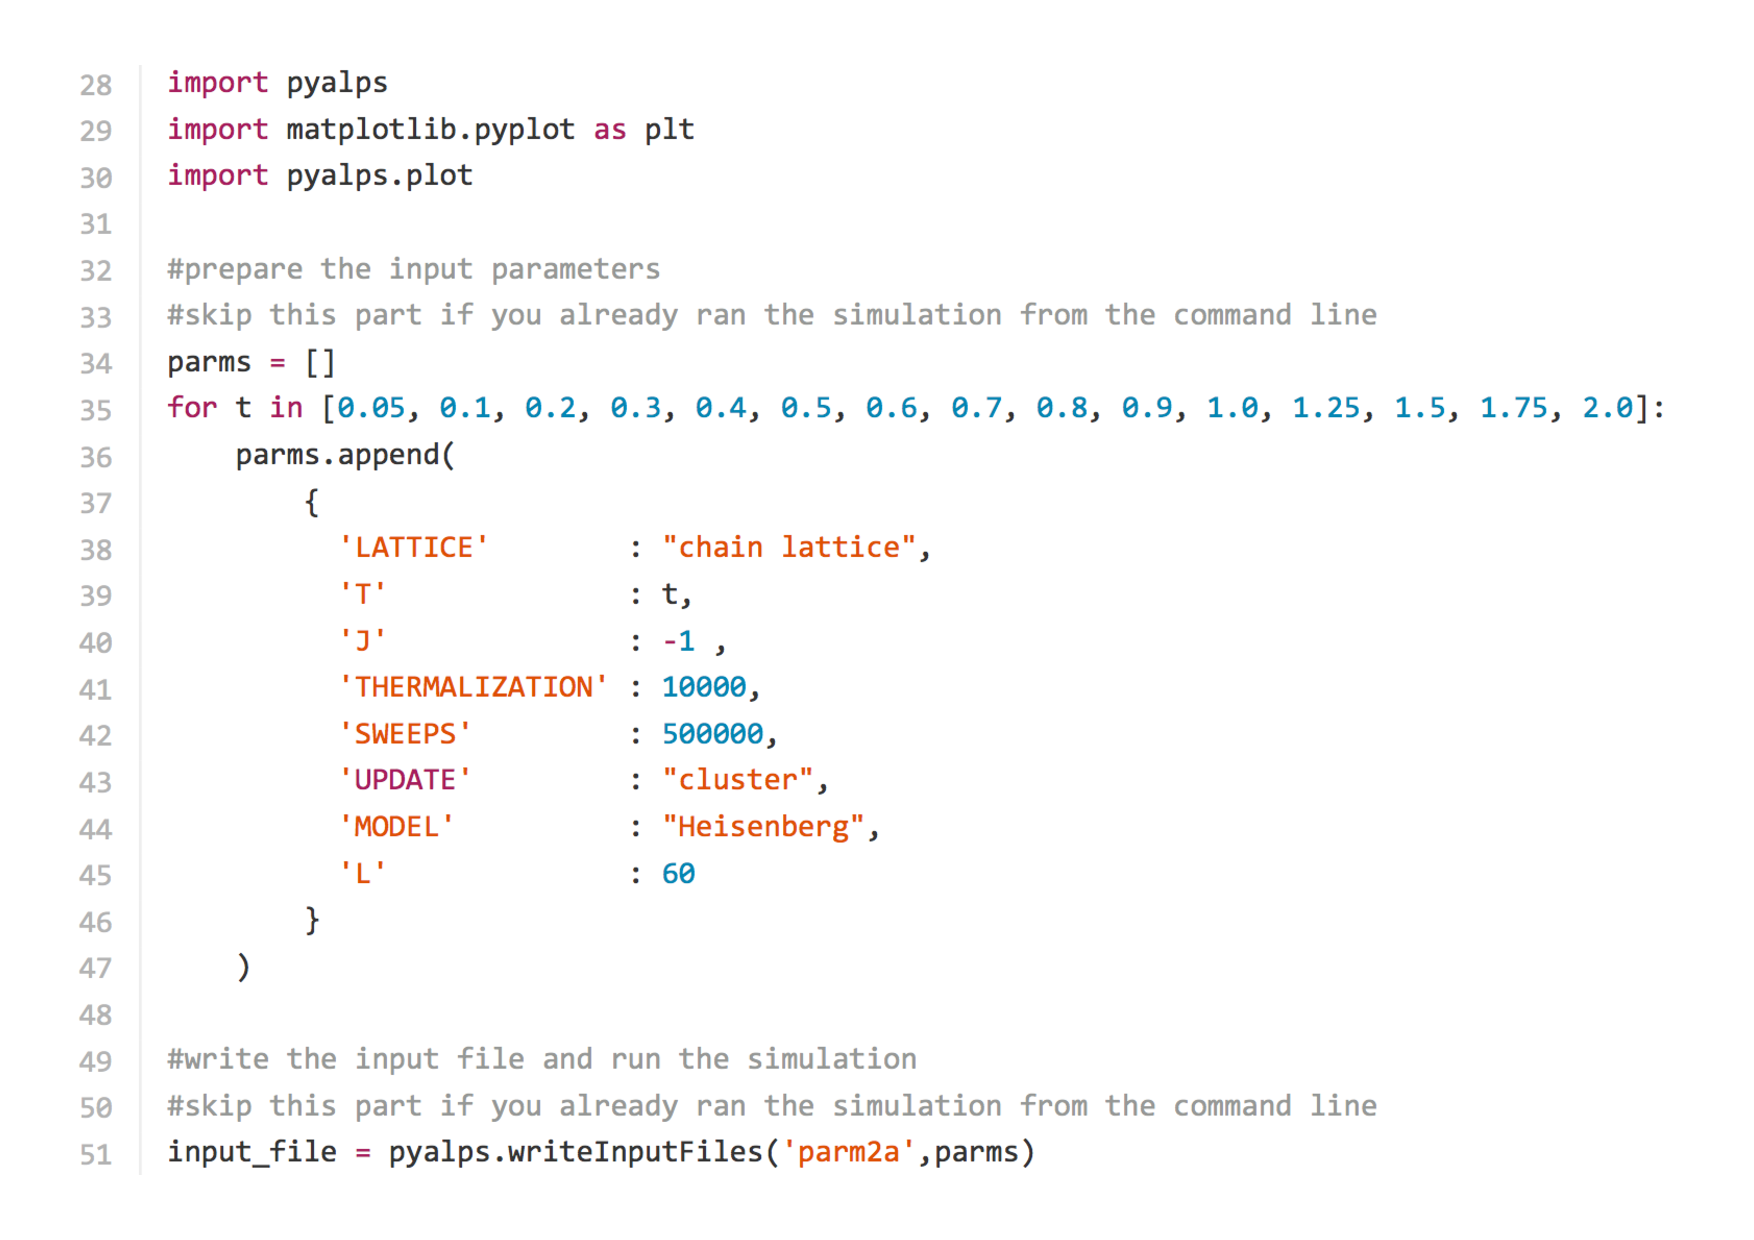
\includegraphics[height=.72\textheight]{tutorial2a-1.pdf}
    %\end{center}
  \end{enumerate}
\end{frame}

\begin{frame}[t,fragile]{Two ways to prepare input files}
  \begin{enumerate}
    \setlength{\itemsep}{1em}
    \setcounter{enumi}{1}
  \item prepare parameter file in text-base simplified format and transform into XMLs by {\tt parameter2xml} tool: ex) parameter2xml myjob
    \begin{center}
      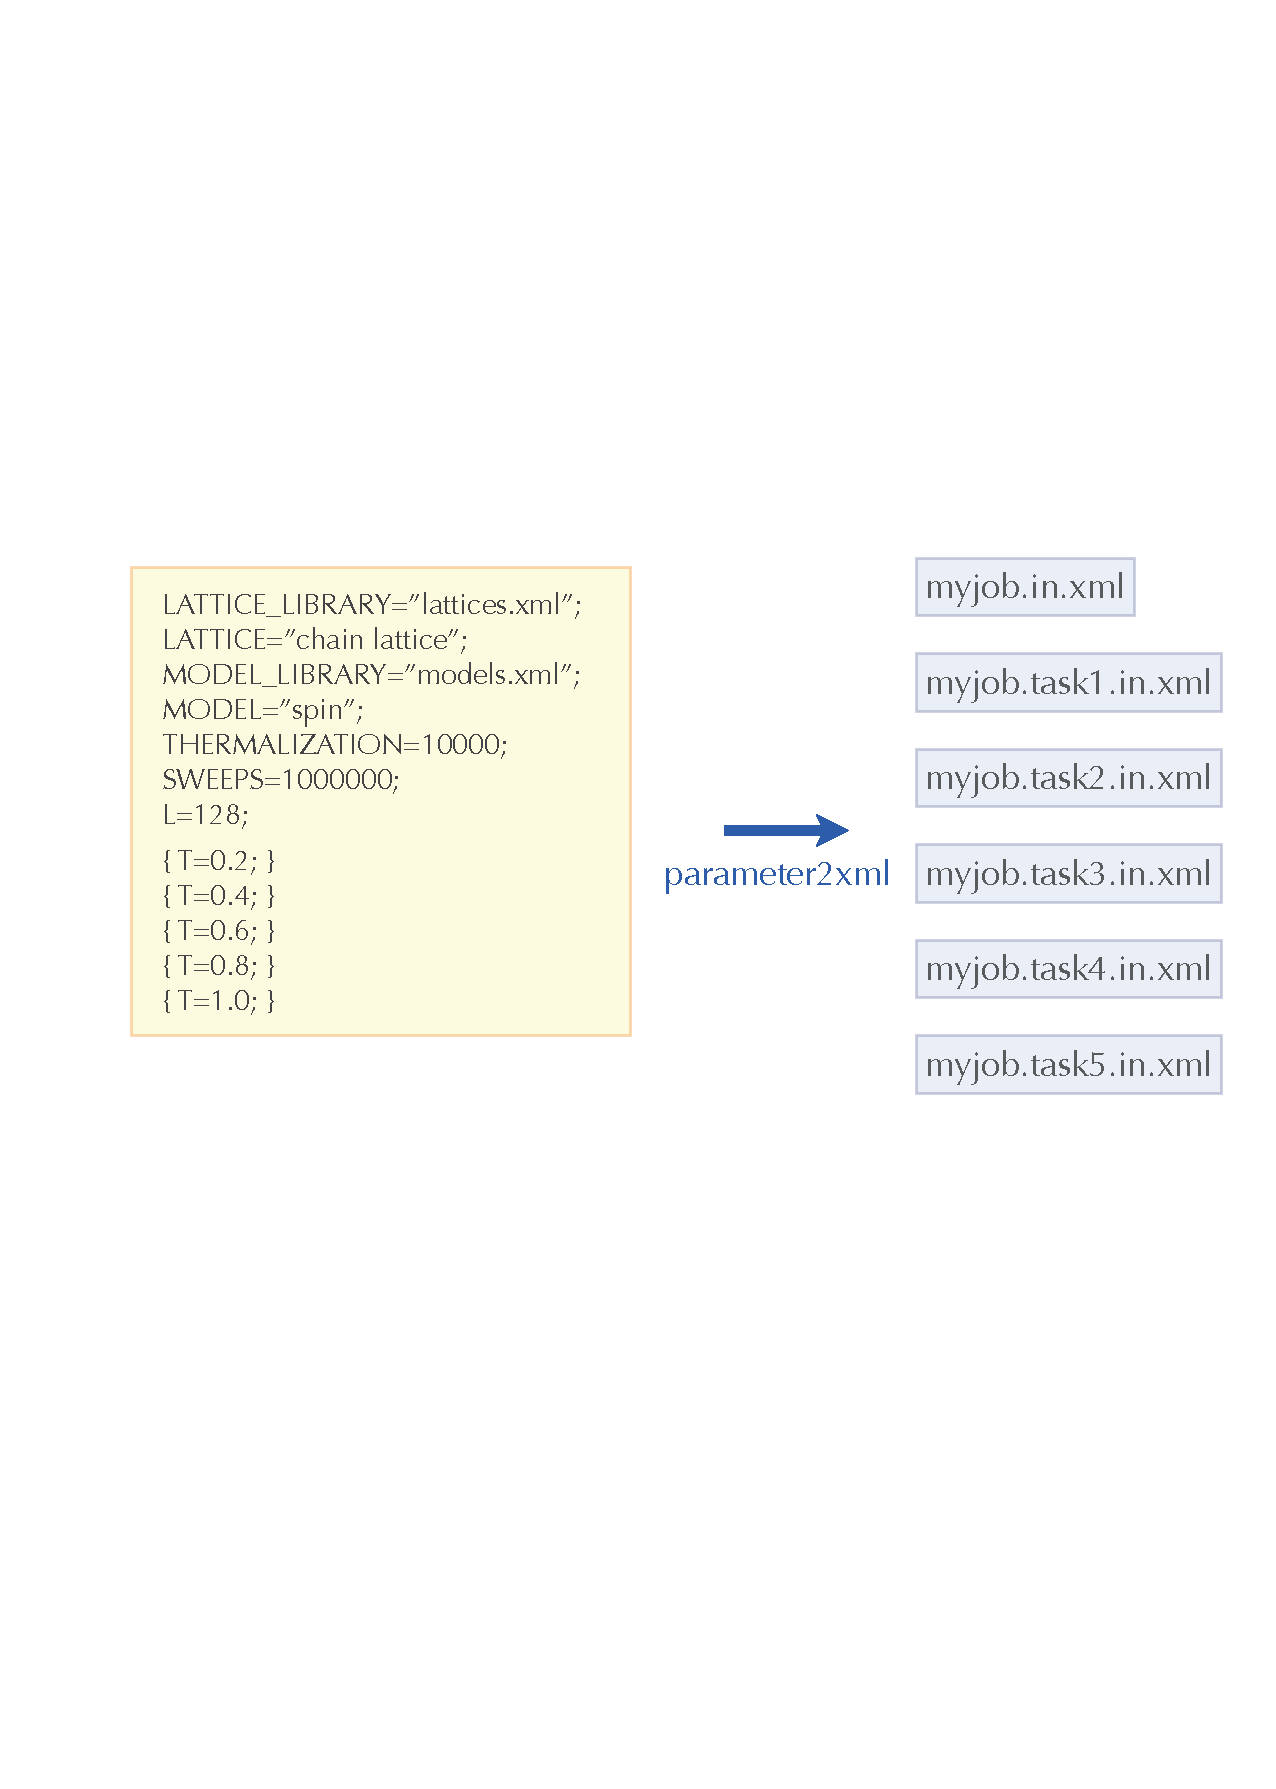
\includegraphics[height=.6\textheight]{simulation4.pdf}
    \end{center}
  \end{enumerate}
\end{frame}

\begin{frame}[t,fragile]
  \frametitle{Simplified parameter file format}
  \begin{columns}[T]
    \begin{column}{.6\textwidth}
      \begin{itemize}
        %\begin{itemize}
        \item New line, semicolon, or comma for separating key-value pairs
        \item Brakets (\{ \}) represents each parameter set
        \item Common parametes before brackets (\{ \})
        \item Arithmetic operations and elementary functions (sin, cos, exp, etc) can be used
        \item {\tt PI} for $\pi$, {\tt I} for imaginary unit
        \item Comments in C and C++ styles
        \item ``Cirular references'' are not allowed
        %\end{itemize}
      \end{itemize}
    \end{column}
    \begin{column}{.4\textwidth}
    \begin{lstlisting}
LATTICE = "chain lattice";
L = 16,
SEED = 2873
// C++ style comment
SWEEPS = 4096;
THERMALIZATION = SWEEPS/8;
/* C style comment */
{ T = 2; Sq = 2*PI/3; }
{ T = 1.8; }
    \end{lstlisting}
    \end{column}
  \end{columns}
\end{frame}

\begin{frame}[t,fragile]{Specifying lattice and model}
  \begin{itemize}
  \item Special parameters for specifying lattice and model
  \begin{center}
    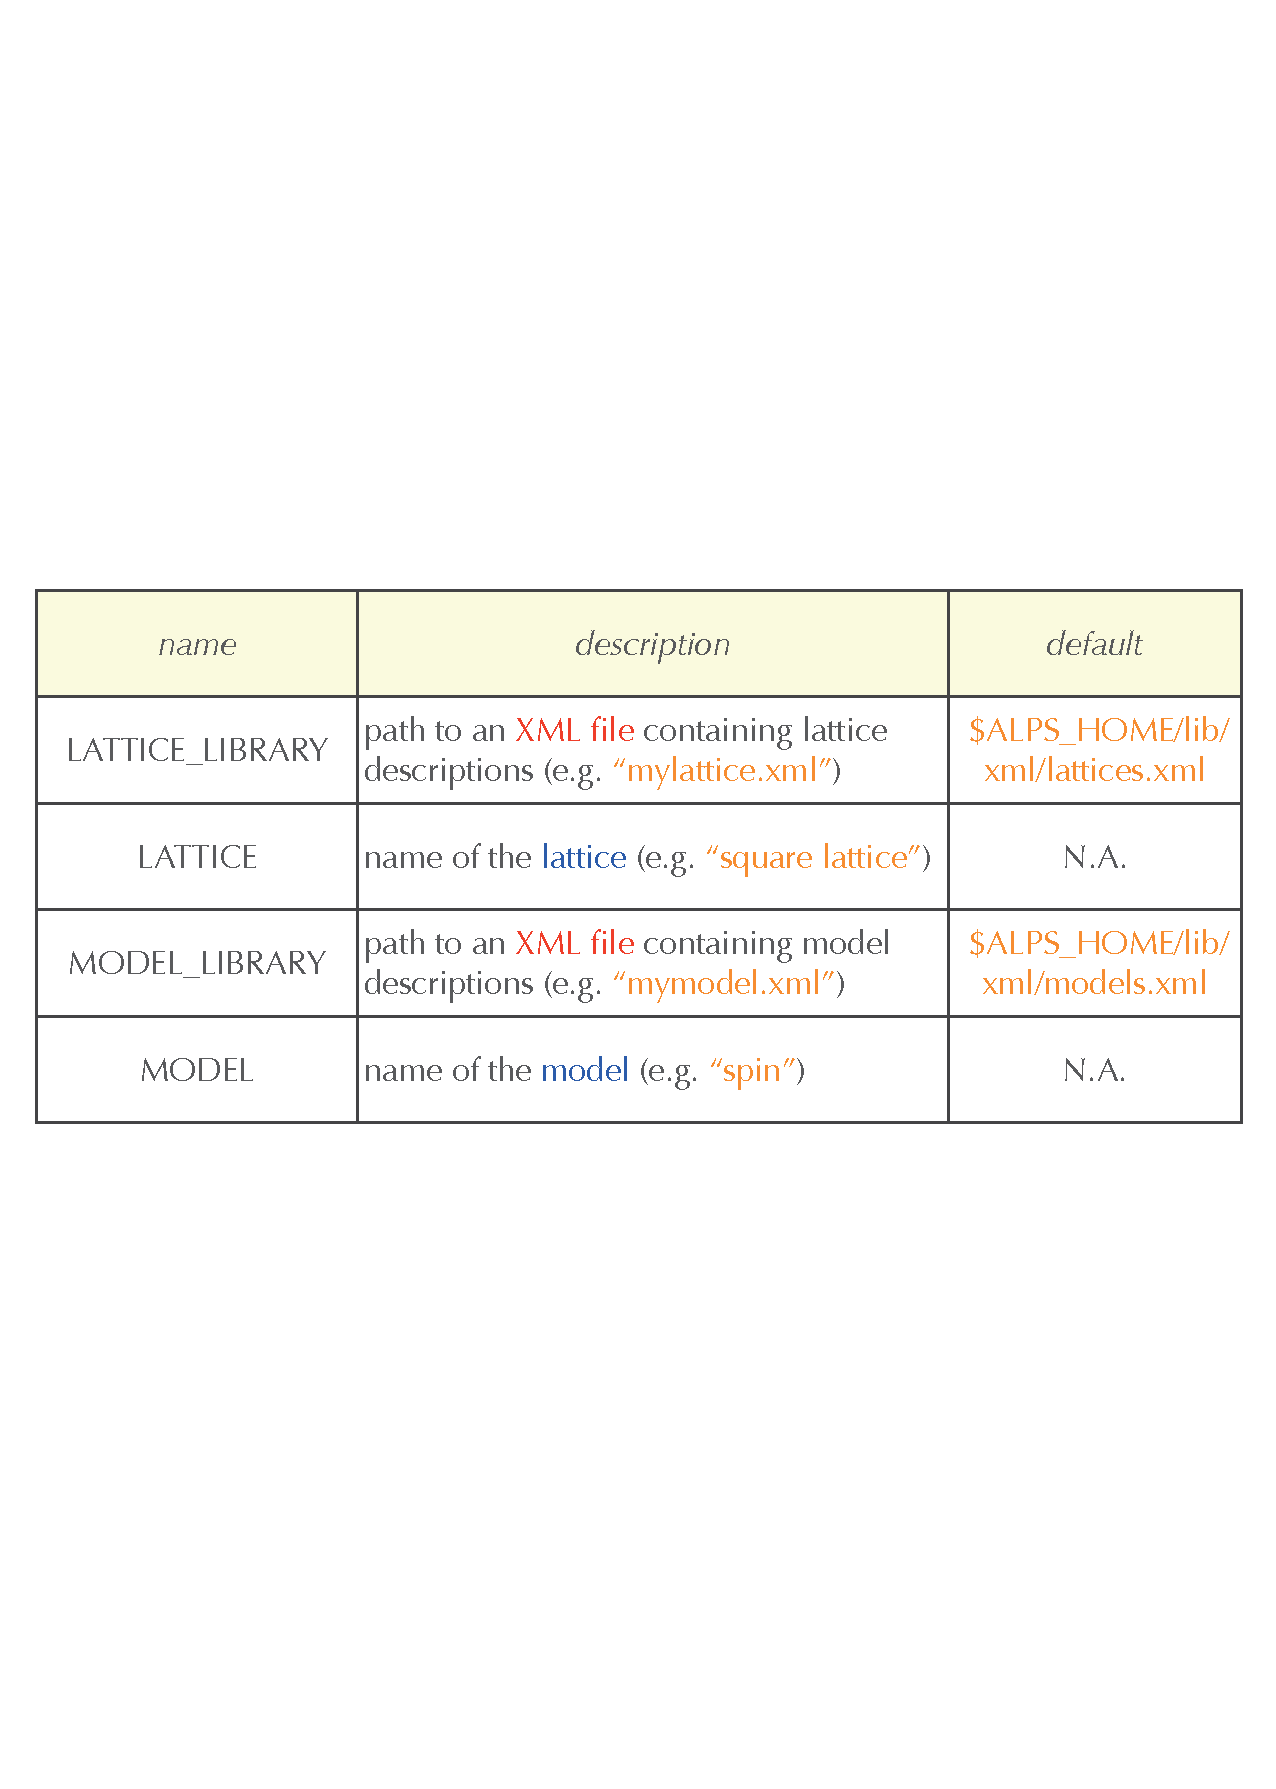
\includegraphics[height=4.5cm]{simulation5.pdf}
  \end{center}
  \end{itemize}
\end{frame}

\section{Running ALPS Applications}
\subsection*{\redm\whiteb\greenb}

\begin{frame}[t,fragile]{Running ALPS applications}
  \begin{enumerate}
  \item from Python script: ex) \href{https://github.com/cmsi/alps-tutorial/blob/tutorials/tutorials/mc-02-susceptibilities/tutorial2a.py}{tutorial2a.py}
    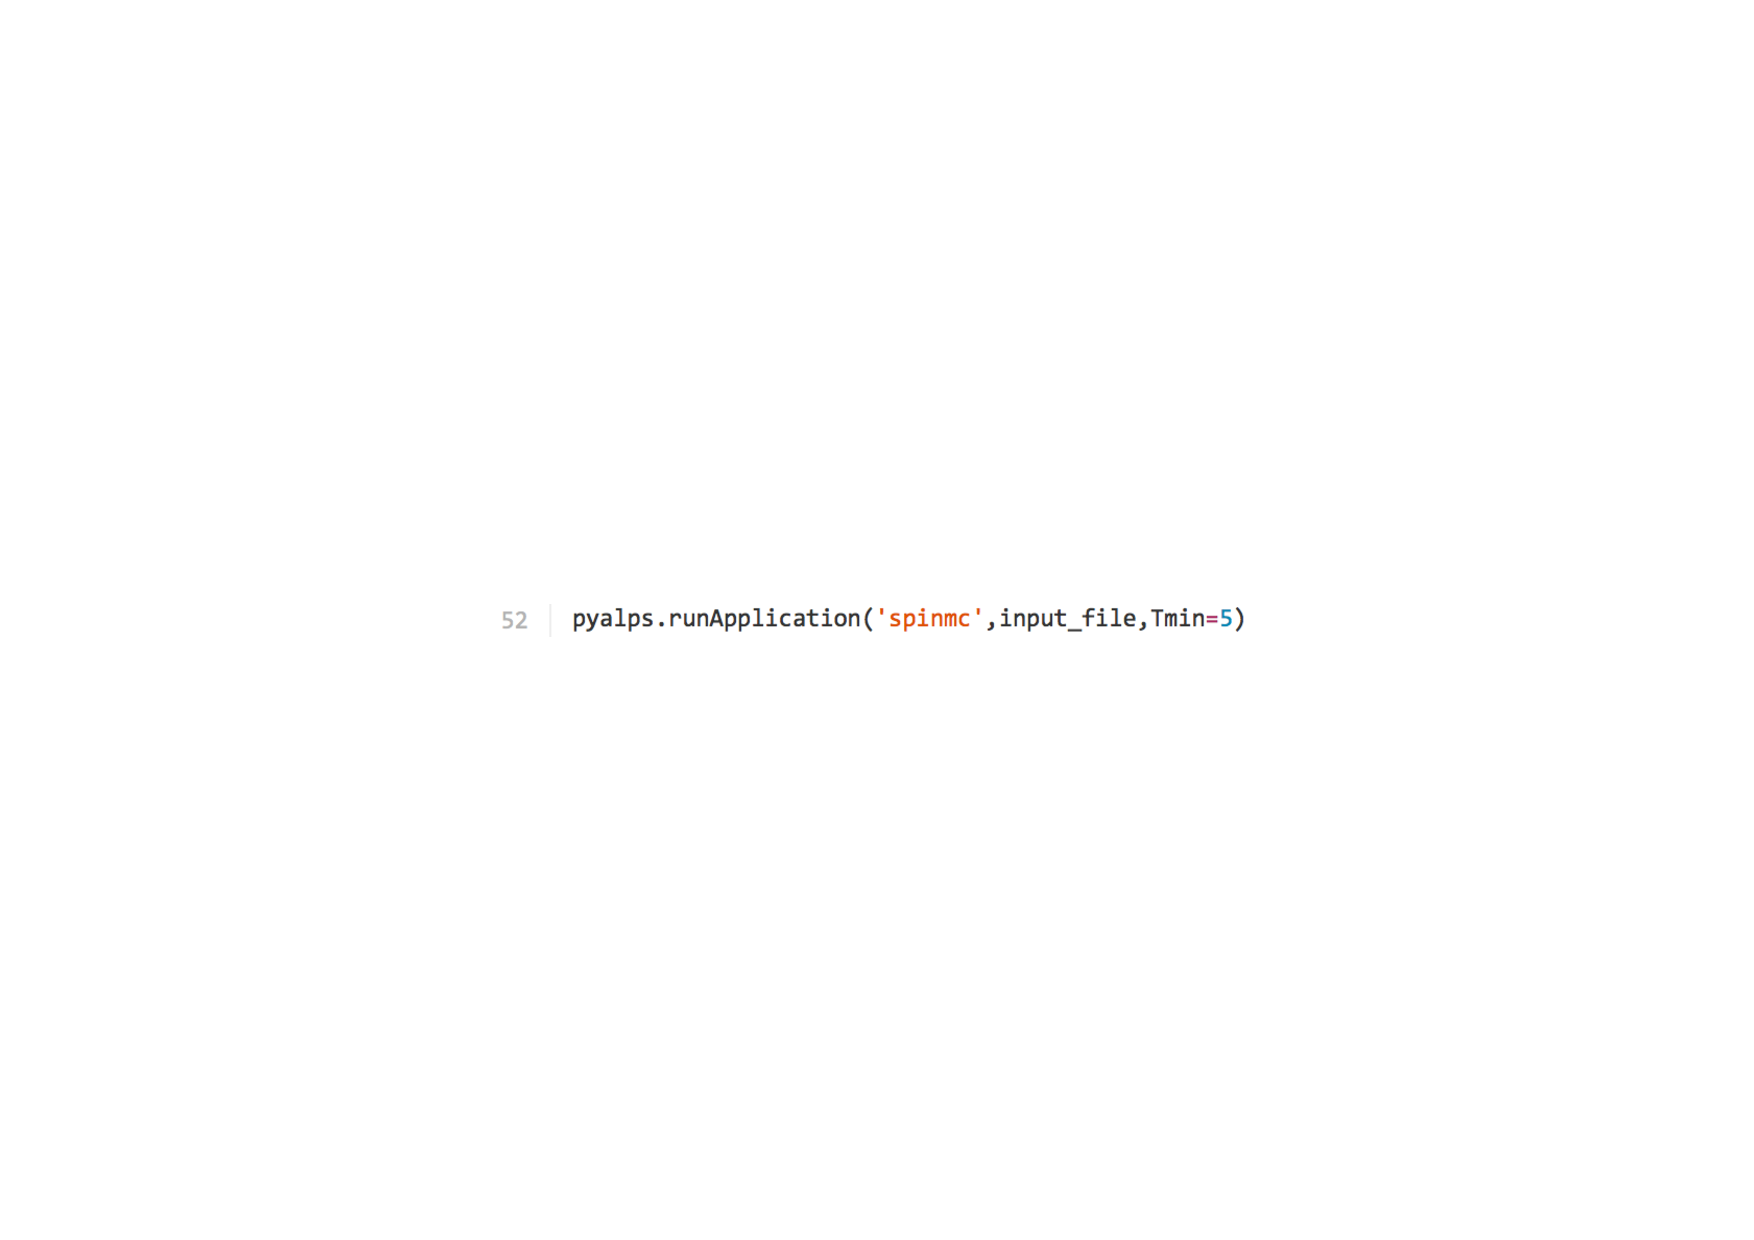
\includegraphics[height=.08\textheight]{tutorial2a-2.pdf}
  \item from command line
\begin{lstlisting}
$ spinmc --Tmin=5 param2a.in.xml
\end{lstlisting}
  \item parallel (MPI) execution (parameter parallelization)
\begin{lstlisting}
$ mpirun -np 8 spinmc --Tmin=5 --mpi param2a.in.xml
\end{lstlisting}
  \end{enumerate}
\end{frame}

\section{Plotting Simulation Results}
\subsection*{\redm\whiteb\greenb}

\begin{frame}[t,fragile]{Plotting simulation results}
  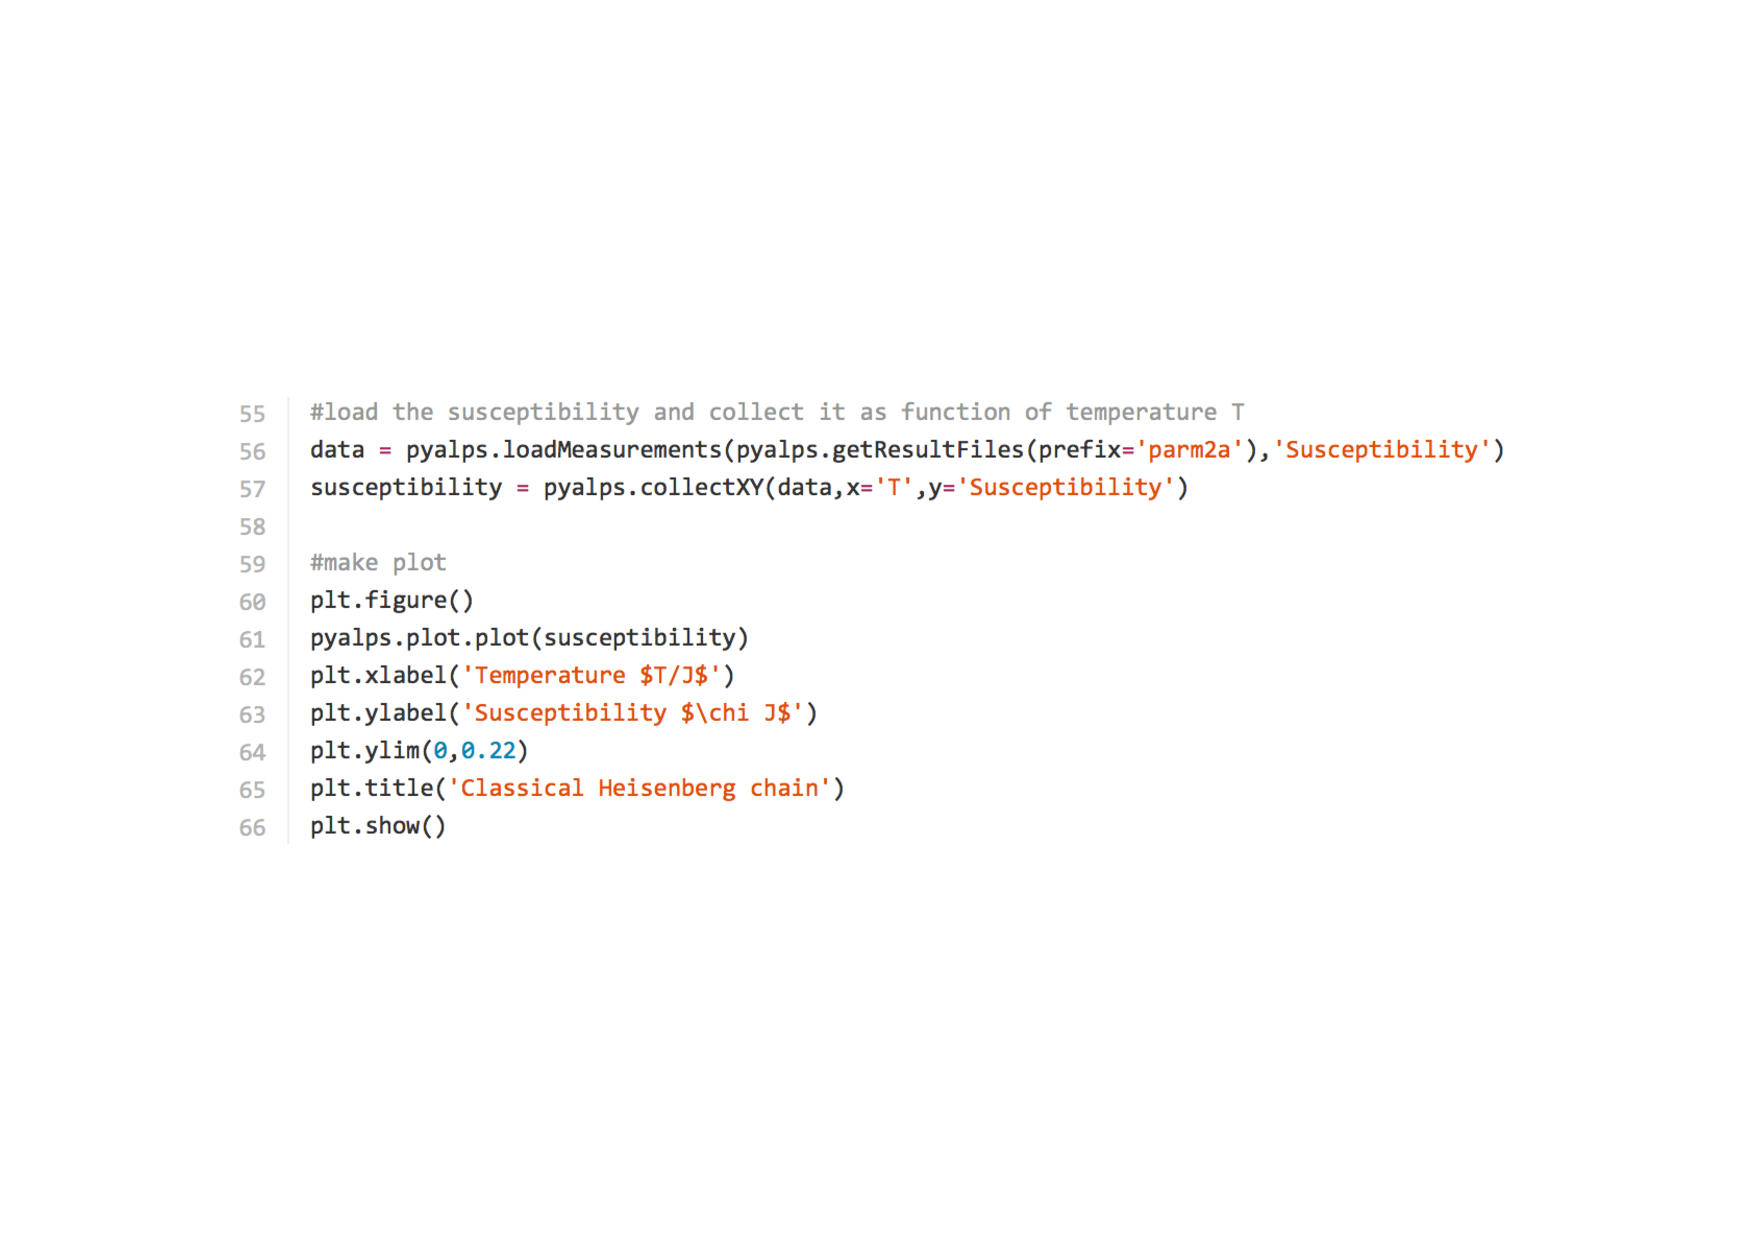
\includegraphics[height=.5\textheight]{tutorial2a-3.pdf}
  \begin{itemize}
  \item If you want to execute Python command row by row on termial, {\color{red}\tt ipython} is more convenient than {\tt python} (tab completion, command history, etc)
  \item Use {\color{red}\tt plt.ion()} to reflect plot commands immediately.
  \end{itemize}
\end{frame}

\begin{frame}[t,fragile]{Three ways to get the list of physical quantities}
  \begin{enumerate}
    \setlength{\itemsep}{1em}
  \item Read \href{http://alps.comp-phys.org/mediawiki/index.php/ALPS_2_Documentation:Overview}{ALPS applications reference documentation}: ex)
    \begin{itemize}
    \item spinmc: {\footnotesize \href{http://alps.comp-phys.org/mediawiki/index.php/Documentation:ClassicalMCSimulations}{http://alps.comp-phys.org/mediawiki/in...}}
    \item loop: {\footnotesize \href{http://exa.phys.s.u-tokyo.ac.jp/en/projects/alps-looper}{http://exa.phys.s.u-tokyo.ac.jp/en/p...}}
    \end{itemize}
  \item Write your own Python script: ex) \href{https://gist.github.com/wistaria/71cb8d7a22f45bfe256d}{list-measurements.py}
    \lstset{language={Python},basicstyle=\small}
\begin{lstlisting}
import pyalps
data = pyalps.loadMeasurements(
       pyalps.getResultFiles(prefix='parm2c'))
{ item.props['observable'] for item in pyalps.flatten(data) }
\end{lstlisting}
  \item (advanced) Use h5dump utility to peek at the contents of *.h5 files
  \end{enumerate}
\end{frame}

\section{Further Tutorials}
\subsection*{\redm\whiteb\greenb}

\begin{frame}[t,fragile]{Still hungry?}
  \begin{itemize}
  \item The following lessons can be done easily by changing parameter file:
    \begin{itemize}
    \item More temperature points?
    \item System size dependence?
    \item Spin-1 chain?
    \item Ising (easy-axis) anisotropy?
    \item Other lattices, such as square lattice, etc?
    \end{itemize}
  \item More tutorials on ED, MC, QMC, DMRG, DMFT are available at ``\href{http://alps.comp-phys.org/mediawiki/index.php/ALPS_2_Tutorials:Overview}{ALPS Tutorials}''!
  \item To define your special lattices and/or models, visit at \href{http://alps.comp-phys.org/mediawiki/index.php/Tutorials:LatticeHOWTO}{ALPS Lattice HowTo} and \href{http://alps.comp-phys.org/mediawiki/index.php/Tutorials:ModelHOWTO}{ALPS Model HowTo}.
  \end{itemize}
\end{frame}

\begin{frame}[t,fragile]{ALPS lattice tutorials}
  \href{http://alps.comp-phys.org/mediawiki/index.php/Tutorials:LatticeHOWTO}{ALPS Lattice HowTo} \\
  \begin{itemize}
    \item \href{http://alps.comp-phys.org/mediawiki/index.php/Tutorials:LatticeHOWTO:SimpleGraphs}{How to specify a simple graph in terms of vertices and edges}
    \item \href{http://alps.comp-phys.org/mediawiki/index.php/Tutorials:LatticesAndUnitCells}{How to specify lattices and unit cells}
    \item \href{http://alps.comp-phys.org/mediawiki/index.php/Tutorials:LatticesAndGraphs}{How to specify graphs corresponding to a lattice with a unit cell}
    \item \href{http://alps.comp-phys.org/mediawiki/index.php/Tutorials:LatticeHOWTO:Library}{How to create a library of lattices and graphs}
    \item \href{http://alps.comp-phys.org/mediawiki/index.php/Tutorials:LatticeHowto:CheckLattice}{How to check a graph generated from a lattice definition}
  \end{itemize}
\end{frame}

\begin{frame}[t,fragile]{ALPS model tutorials}
  \href{http://alps.comp-phys.org/mediawiki/index.php/Tutorials:ModelHOWTO}{ALPS Model HowTo} \\
  \begin{itemize}
  \item \href{http://alps.comp-phys.org/mediawiki/index.php/Tutorials:ModelHOWTO#The_default_model_libary_file}{The default model libary file}
  \item \href{http://alps.comp-phys.org/mediawiki/index.php/Tutorials:ModelHOWTO#General_structure_of_a_model_library_file}{General structure of a model library file}
  \item \href{http://alps.comp-phys.org/mediawiki/index.php/Tutorials:ModelHOWTO#The_basis_of_a_single_site}{The basis of a single site}
  \item \href{http://alps.comp-phys.org/mediawiki/index.php/Tutorials:ModelHOWTO#The_basis_of_the_full_lattice_model}{The basis of the full lattice model}
  \item \href{http://alps.comp-phys.org/mediawiki/index.php/Tutorials:ModelHOWTO#Quantum_operators}{Quantum operators}
  \item \href{http://alps.comp-phys.org/mediawiki/index.php/Tutorials:ModelHOWTO#Hamiltonian_descriptions}{Hamiltonian descriptions}
  \end{itemize}
\end{frame}

\end{document}
